\documentclass{article}

\usepackage{Sweave}
\begin{document}
\Sconcordance{concordance:accuracy.tex:accuracy.Rnw:%
1 2 1 1 0 35 1 1 21 3 0 1 1 9 0 1 12 2 0 1 1 10 0 1 4 3 1 1 6 1 3 2 1 1 %
6 1 3 2 1}


\title{Accuracy}

\author{Mc}
\maketitle
\section*{Introduction}
In plots we recast the results of simulations in terms of accuracy. We compute the accuracy of each method (continous or categorical), for each level of \(\rho\) (see below) by computing the  the following quantities:
\begin{itemize}
  \item false positive (FP)  runs with  with a significant test under a true null hypothesis
  \item true positive (TP) runs with a significant test under a false null-hypothesis 
  \item true negative (TN) runs  with a nonsignificant result under a true null-hypothesis
  \item false negative (FN) runs with a nonsignificant result under a false null-hypothesis

\end{itemize}

Plots to be produced:
\begin{itemize}
  \item Sensitivity for all 4 of the decision possibilities (continuous ignoring categorical, categorical ignoring continuous, both, either), with X axis being rho (Figure 1)
  \item PPV for the 4 decision possibilities, with X axis being rho (Figure 2)
  \item Bar chart with the specificity for the 4 decision possibilities
  \item Bar chart with the NPV (aggregated over rho) for the 4 decision possibilities
\end{itemize}

\section*{Setup}
\subsection*{Model}
Two continuous latent variables (\(\eta\) and \(\xi\) ) are created with N cases, sharing a correlation equal to \(\rho\). A measure \(x\) of \(\xi\) is created with reliability \(rel\), and then  is dichotomized accordingly to \(p\) \(1-p\) into \(c\). The correlations \( r_pe=r(\eta,x) \)  and \( r_pb=r(\eta,c) \) are computed, their p-value and significance (at .05) is recorded.
\subsection*{Design}
\(\rho=(0,.1,.2,.3,.4,.5,.6,.7) \)
\(rel=(0.3, 0.4 ,0.5, 0.6, 0.7 ,0.8 0.9) \) 


\subsection*{Computation of quantities}

\begin{itemize}
  \item Continuous false positive (FP\_C)  freq of runs with continuous test p.<.05 and \(\rho\)=0  
  \item Continuous true positive (TP\_C)  freq of runs with continuous test p.<.05 and \(\rho\)>0
  \item Continuous true negative (TN\_C)  freq of runs  with continuous test p.>=.05 and \(\rho\)=0
  \item false negative (FN\_C)  freq of runs  with continuous test p.>=.05 and \(\rho\)>0
\end{itemize}

The same quantities are computed for the categorical indicator (*\_S).

\begin{Schunk}
\begin{Soutput}
Accuracy for continuous indicator
\end{Soutput}
\begin{Soutput}
  rho    SENS_C    SPEC_C
1 0.1 0.1050000 0.9507143
2 0.2 0.2511429 0.9507143
3 0.3 0.4511429 0.9507143
4 0.4 0.6090000 0.9507143
5 0.5 0.7204286 0.9507143
6 0.6 0.7974286 0.9507143
7 0.7 0.8618571 0.9507143
\end{Soutput}
\begin{Soutput}
Accuracy for categorical indicator
\end{Soutput}
\begin{Soutput}
  rho     SENS_S    SPEC_S
1 0.1 0.08414286 0.9498571
2 0.2 0.17957143 0.9498571
3 0.3 0.33785714 0.9498571
4 0.4 0.47128571 0.9498571
5 0.5 0.61057143 0.9498571
6 0.6 0.70114286 0.9498571
7 0.7 0.77900000 0.9498571
\end{Soutput}
\begin{Soutput}
   con.sig cat.sig rho freq
1        0       0 0.0 6438
2        1       0 0.0  211
3        0       1 0.0  217
4        1       1 0.0  134
5        0       0 0.1 6026
6        1       0 0.1  385
7        0       1 0.1  239
8        1       1 0.1  350
9        0       0 0.2 4955
10       1       0 0.2  788
11       0       1 0.2  287
12       1       1 0.2  970
13       0       0 0.3 3590
14       1       0 0.3 1045
15       0       1 0.3  252
16       1       1 0.3 2113
17       0       0 0.4 2570
18       1       0 0.4 1131
19       0       1 0.4  167
20       1       1 0.4 3132
21       0       0 0.5 1795
22       1       0 0.5  931
23       0       1 0.5  162
24       1       1 0.5 4112
25       0       0 0.6 1286
26       1       0 0.6  806
27       0       1 0.6  132
28       1       1 0.6 4776
29       0       0 0.7  863
30       1       0 0.7  684
31       0       1 0.7  104
32       1       1 0.7 5349
\end{Soutput}
\begin{Soutput}
Accuracy for BOTH indicators significant
\end{Soutput}
\begin{Soutput}
  rho     SENS_B    SPEC_B
1 0.1 0.04761905 0.9808571
2 0.2 0.12170640 0.9808571
3 0.3 0.23186656 0.9808571
4 0.4 0.30911962 0.9808571
5 0.5 0.37005040 0.9808571
6 0.6 0.40557065 0.9808571
7 0.7 0.43315248 0.9808571
\end{Soutput}
\begin{Soutput}
Accuracy for EITHER indicators significant
\end{Soutput}
\begin{Soutput}
  rho    SENS_E    SPEC_E
1 0.1 0.1391429 0.9197143
2 0.2 0.2921429 0.9197143
3 0.3 0.4871429 0.9197143
4 0.4 0.6328571 0.9197143
5 0.5 0.7435714 0.9197143
6 0.6 0.8162857 0.9197143
7 0.7 0.8767143 0.9197143
\end{Soutput}
\end{Schunk}

\subsubsection*{Figure 1: Sensitivity of the two methods}

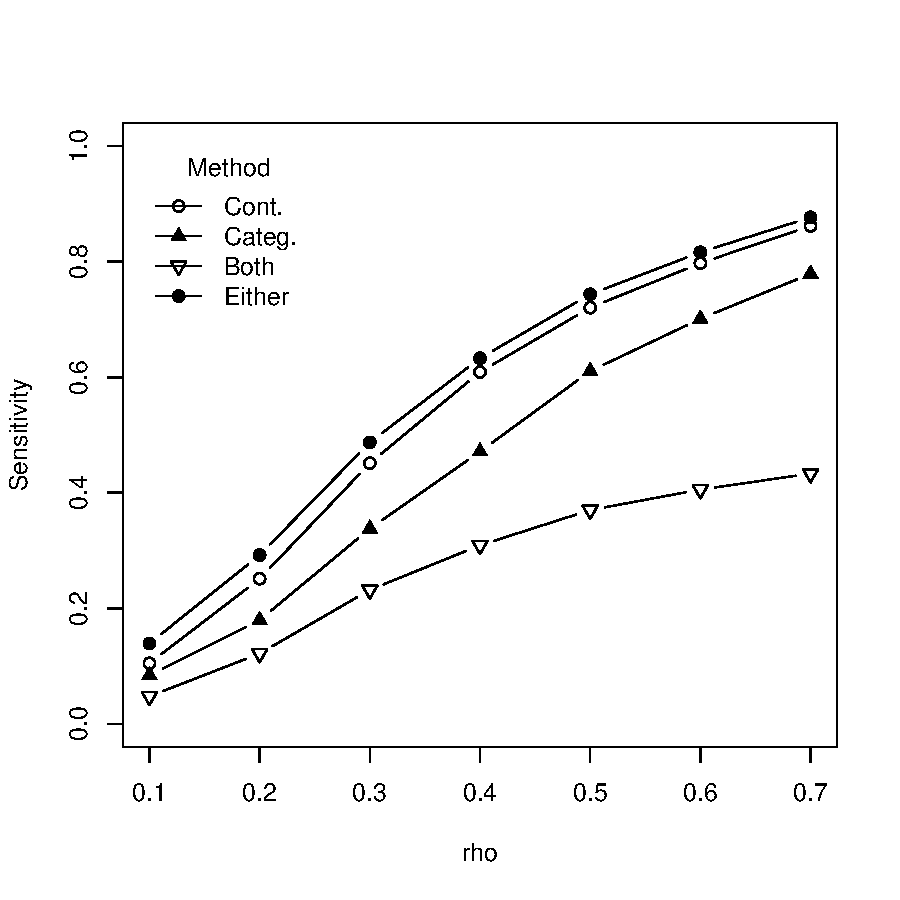
\includegraphics{accuracy-dd}



\end{document}
